%!TEX root = dissertation.tex

\chapter*{About this project}
\paragraph{Abstract}

Dúchas Na Gaillimhe ( Galway Civic Trust ) along with Tourism Ireland carry out walking tours of Galway city to inform visitors of Galway's long and rich history. One of the walks they offer tourists during the summer months is a medieval walking tour of Galway city. This walk visits seven locations starting in Galways Latin Quarter. However, this limits visitors to attending guide-lead tours at specific times as well as only being available frequently during the summer tourist season.

This project aims to deliver a solution which helps tourists visiting Galway city to take the medieval walking tour of Galway at any time, without the need of a guide and will be available at any time of the year. If the tourist wishes to seek further information they can drop into Galway Civic Trust's office which is located at one of the seven stops along the route - at the Hall Of the Red Earl.

The proposed solution will comprise a mobile phone application which will allow users to be guided around Galway city. It will show the user their current location and guide them to the destination they wish to reach. On arrival at the destination, the app provides the user with information and images about the location. A user can get additional information if they so wish. There will also be a web application used by Galway Civic Trust personnel to update the information on the application periodically and make it automatically available to all new and existing app users.

\paragraph{Authors}
Sarah Carroll, Abigail Culkin
B.Sc.(Hons) in Software Development

\chapter{Introduction}

At the beginning of Year 4 in Software Development at GMIT, the authors were given the opportunity to work on the Medieval walking tour project for an external small/medium Enterprise organised through GMIT. The idea of the project is based on the problem that medieval walking tours of Galway city are not always available for tourists at convienient times and infrequently outside the main summer season. 


The purpose of this Final Year Project is to build an application using new technologies that the developers have never used before. Therefore, it allows for research to be done and learn up and coming technologies and learn new ways of developing software. The front-end technology being used is Flutter. It will be connected to a backend server running on Google cloud platform and within this a MongoDB Flask Database which uses docker. Working with Galway Civic trust allowed for an application to be made that is missing from the market place for Galway tourism. This application will be useful and easy to use for customers and the company will benefit from this.  This way the authors will be able to show they have worked with an outside source and have a fully functioning app that will satisfy what was asked of them.


It will be explained the technologies used and why we used them throughout. The research and development will all be detailed and allow others to understand why specific software was chosen. This project is done using technologies that have not been used together too often. This means any problems faced or certain aspects found to be new will be documented along with the development.
\section{Context}

\subsection{Context of the Project}

The context of this project revolves around the use case of being a tourist in Galway city, wishing to find out more information about the city's history. Opening the app on your phone, viewing your location in relation to the locations on the guided tour. This application prevents the user getting lost and gives them accurate information about each location.  The information on the application was provided by Galway Civic Trust and is the same information a tourist gets on the guided walking tours. Reading the data and retrieving images from the database needs to be very fast, as any delayed hang in performance could lead to a bad user experience.

The project will be developed as a Cross-Platform application which provides users with images, information and a map of Galway city and the seven medieval stops along the tour. Users of the application can get their location in relation to the exact location of the points of the tour at any given time. When the user decides they wish to learn more information about a specific location, the user can retrieve images and text about the location on the application. Along with the  mobile application a web application will be developed for use by Galway Civic Trust personnel to update, delete or add information to the tour database.

\section{Objectives} 


The project will require a number of objectives to be accomplished in order to provide a solution that works and is suitable for the use of Galway Civic Trust. 

\begin{itemize}
\item A Mongo database will be used to store the text and images which appear in the application. This database will need to be setup and hosted in such a way that it can be accessed from clients on the web. The database will be hosted on Amazon Web Services Cloud.

\item A client application will be the main product / asset for the project. This application will be able to locate the user via the GPS on their mobile device. The app will then show the user the locations of each point on the tour. This will provide the user an idea of how long they are from the chosen point and will allow them to see when they have reached their destination.

\item Another requirement is to develop a web application for the use of the company to allow them to modify the information shown to the user.

\item Using Google Maps api within the mobile application to show the user their location along with the specific points of the tour.

\item Pull information from the Mongo DB using node.js


\end{itemize}
\section{Overview}

Each Chapter of this paper will contain different details regarding the project. 

The Methodologies section will describe the way in which decisions were made about the project. The way in which software development and research methodology was addressed. The aids used to help working in a team will also be discussed.

The Technology Review will go into more detail on the different technologies used throughout the project and the reasoning for choosing each. An example of these technologies are node.js.

The System Design will provide a detailed explanation of the overall system architecture. This is the "HOW" of the project.

The System Evaluation compares the project against the initial objectives set out in the introduction. This will also include how new features could be included for future use by the customer.

The conclusion briefly summarises the context and objectives of the project.

\chapter{Methodology}

\section{Selection Criteria}

During the initial planning of this project, the frames works considered included Ionic, Flutter and Xamarin. The winner was the Flutter framework. This is a new framework introduced by Google. It is built using the Dart programming language. Flutter has multiple benefits including its simplicity to be used for cross platform applications.

Flutter is maintained on a single code base for all platforms. This enables simplicity for testing and reduces development time. For this reason it was chosen over Xamerin framework. Xamerin is a C Sharp based platform. Flutter offers APIs and SDKs for 2D rendering, simulation, gestures, and painting as well as allowing the use of existing Swift, Objective C, and Java code. It comes with Machine Design Widgets, also a Google product. \cite{flutterVsXamarin}

Flutter and Ionic are very similar is what they offer with regards to pre-built components in Ionic and a comprehensive suite of built in widgets in Ionic \cite{ReactVsFlutterVsIonic}. With Ionic, you create a real native app but you do this by creating a web app (with Hyper text markup language, JavaScript and Cascading style sheet) which will be wrapped by a real native app that hosts a web view while Flutter you write Dart code which can be compiled to native code that runs on the target device. The main reasoning for using Flutter over Ionic is that it is new. It is powered by Google and therefore is well documented and although its still in beta testing there are loads of interactive talks online about the upcoming and new features of Flutter. 

\section{Testing and Validation}
Testing is an essential part of any software development life cycle. The importance of testing in software development life cycle is to improve reliability, performance and other important factors.\cite{TestingLifeCycle} Each component of the project can be tested individually.
 
\subsection{Unit Tests}

Unit tests are individual tests to check functions,methods or classes. A test library is imported into the flutter application. The developer/tester can run the unit tests from the terminal to check for success or failure. Unit tests can test that visual aspects of the application are working correctly along with connection to database.

\subsection{Widget Testing}

A widget test tests a single widget. Testing a widget involves multiple classes and requires a test environment that provides the appropriate widget life cycle context. \cite{testing}. It tests that the widget user interface performs as expected both visually and its interactions. A widget should be able to check for user input and check for responses for the user based on actions performed. It is similar to unit testing because it tests the environment and is usually created to test certain actions alone.

\subsection{Integration Testing}

Integration testing is used to test the flutter application in whole. This tests that each function checked in unit and widget tests also work when Incorporated with the remainder of the application. Integration testing is also used to test the performance of the application. This was done to test that the application could retrieve information from the database by many users simultaneously. Developers/testers can run the command "flutter driver" which sets uo the test harness, builds and installs the application and runs the integration tests on the application. \cite{IntegrationTest}

\begin{figure}[ht!]
    \centering
 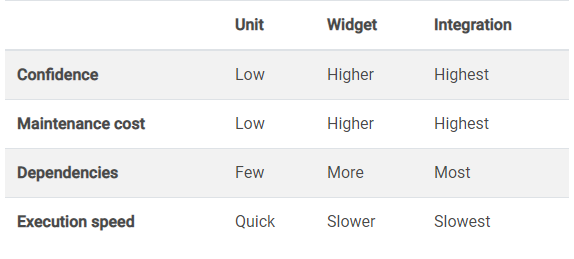
\includegraphics[width=125mm,scale=0.5]{img/Capture.PNG}
\caption{Testing:Types of testing}
\cite{testing}
\label{fig:method}
\end{figure}

\section {Continuous Integration / Continuous Delivery}

Due to this project being produced in conjunction with Galway Civic trust,working closely with Michael Quinn to produce the exact item he wishes to publish is necessary. In order to do this Software engineering techniques are being used to ensure the customer receives exactly whats needed. The main approaches used are test driven development(TDD), behaviour driven development(BDD) and user storyboards.

\subsection{Storyboards}

Storyboards were used to allow the customer give the developers a high level view of expected design of the application. This is done using a blank page and the customer draws a simple representation of what they want to application to look like. This gives the developers a better understanding and idea what needs to be done and can help break down upcoming tasks to be completed. The storyboard used is taken from the agile methodology and is continuously being referred to and brought to each meeting with the customer to ensure every design requirement is clearly met. \cite{StoryBoard}

\subsection{Behaviour Driven Development}

Behaviour driven development is another agile software development methodology. It is designed base what the user wants and how the user explains what the visual display of the application should be. The customer/user gives a list of behaviours they wish the application the be able to accomplish. These simple requests and made into a task or multiple tasks for the developer. When the application is complete the original requirements are made into unit tests.\cite{BDD} 

\subsection{Test Driven Development}

Test Driven Development is based predominantly on unit testing. However they are very different because test driven development is when the unit tests are written before the code has been created. This means the developers are using the unit tests as a guild and the tests alone break down the overall task needing to be completed.The tests will initally fail and the developers write minimal code in order the the tests to pasS. This is process in continuously repeated in order for the application to pass each test. These tests are commonly automated.\cite{TDD}

\section{Project Management}

Project Management is a key element of any task to ensure that the project was laid out correctly and each component part is complete at a given date etc. Because this project was completed by a team it was important both members completed each task. In order to track the project a gantt chart was user. This broke down each step of the project and the expected time limits for each section.










 


